\chapter{Introduction}
\section{Background}
The ability to detect the direction of a sound source is a remarkably intuitive skill possessed by humans and animals.
This capability is facilitated by the use of just two ears, leading to what is essentially an underdefined system.
The uniquely shaped structure of the ears allows the brain to discern subtle differences in sound reception,
enabling the identification of whether a sound originates from the front or behind.
Replicating this natural phenomenon in a technical setup presents a significant challenge,
as the human brain employs complex auditory processing methods honed over a lifetime of learning.

A practical approach to addressing this challenge in sound source localization is the employment of multiple microphones, akin to having more ears.
By strategically arranging these microphones in an array configuration, it becomes feasible to utilize beamforming algorithms to ascertain the direction of a sound source.

With the rising popularity of drones, instances of their misuse have also increased.
This trend has sparked interest in the development of detection and tracking systems for drones.
Utilizing a sound localization system for this purpose offers distinct advantages over other technologies that depend on optical or thermal detection.
Humans often rely on their auditory sense as an initial alert to the presence and location of a drone,
a method that remains effective even in adverse weather conditions where visual sighting is compromised,
or in scenarios where thermal detection is ineffective, such as when a drone is silhouetted against the sun.
Compared to radar-based tracking systems, acoustic drone localization technology is considerably simpler and more cost-effective,
making it an attractive solution for drone detection and tracking.

\newpage
\section{Scope}
The primary objective of this project was to conceptualize and develop a system capable of acoustically pinpointing objects, such as drones.
The inherent limitation of a single microphone array is its ability to determine only the direction of a sound source, not its distance.
Consequently, it became apparent that accurate localization of drones in the three-dimensional space necessitates the integration of multiple microphone arrays.
Each array contributes a directional vector towards the sound source.
The exact position of the object is then deduced by finding the theoretical point of intersection of these vectors, considering the known locations and orientations of each array.
Figure \ref{fig:areal_overview_diagram} illustrates this concept.
\begin{figure}[h!]
	\centering
	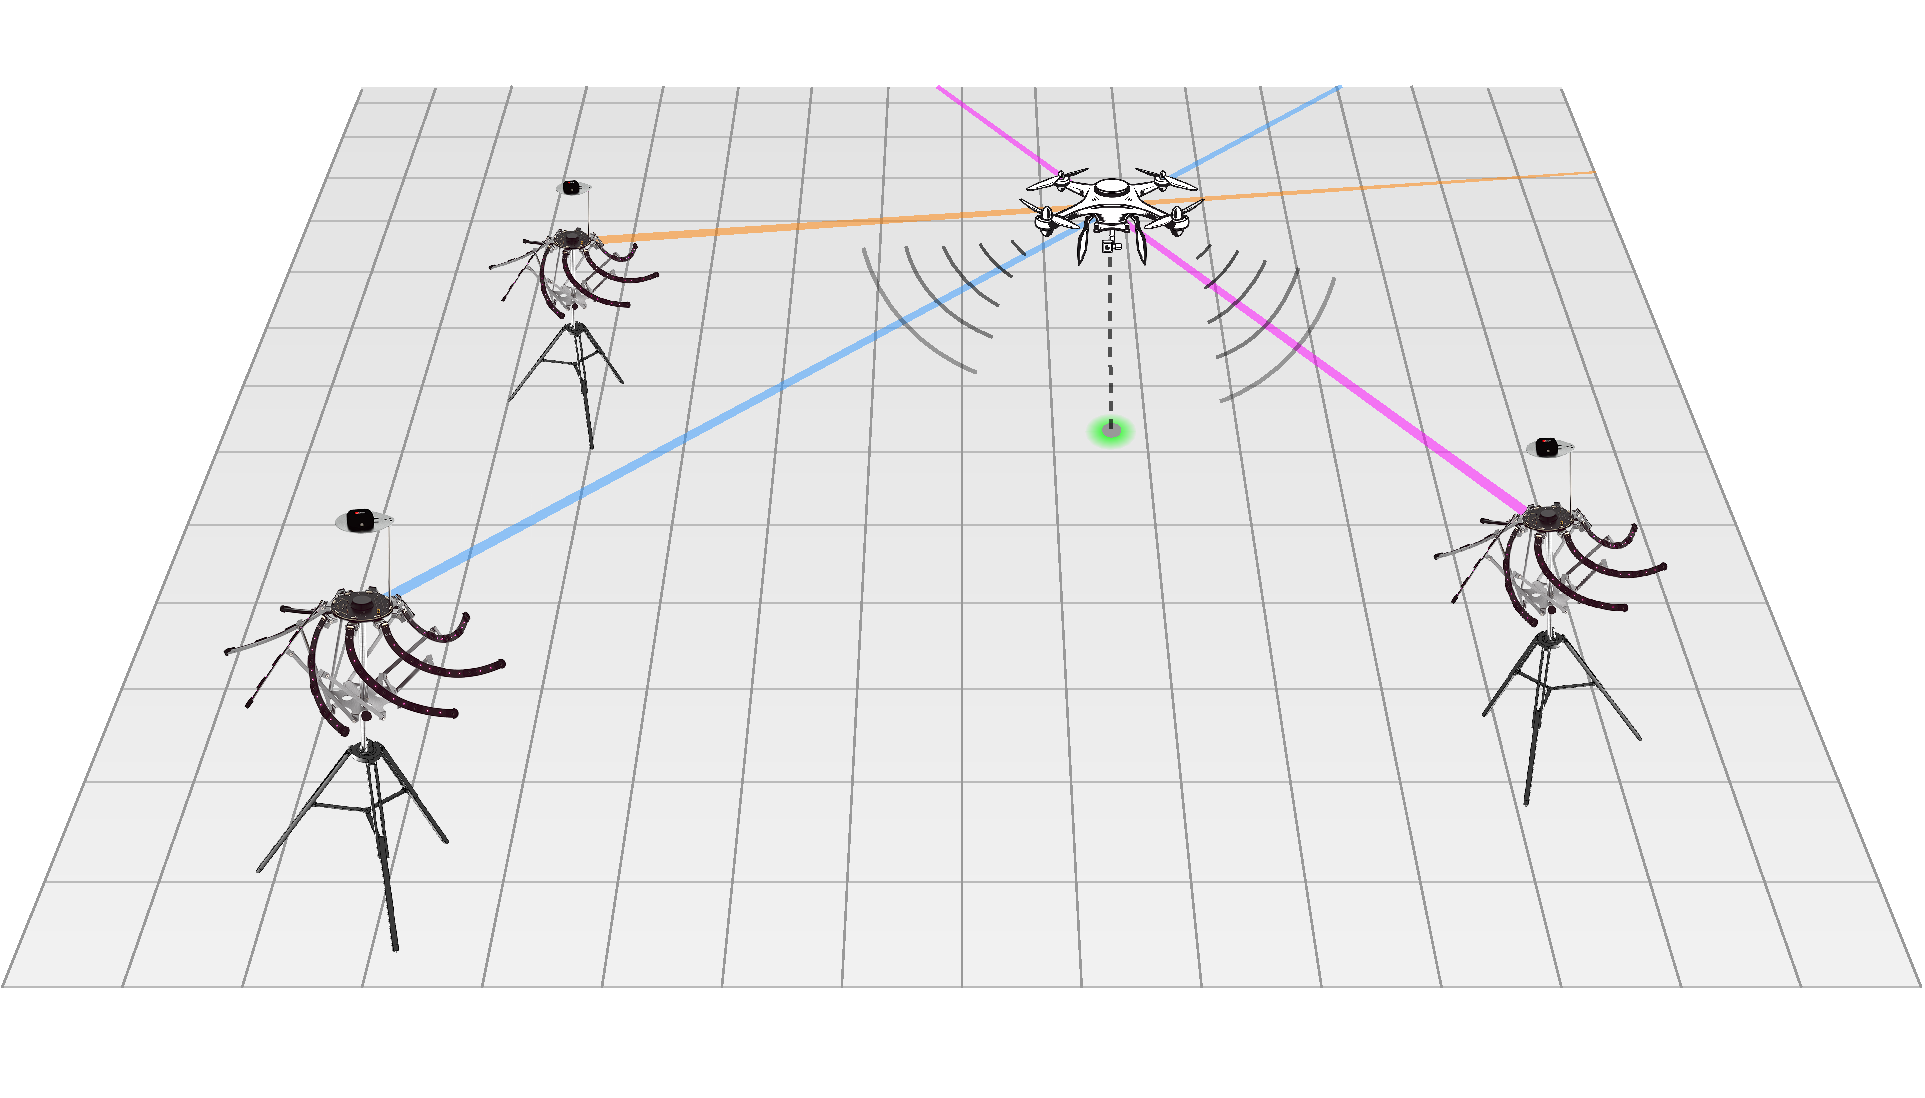
\includegraphics[width=1.0\textwidth, trim={0 -0.1cm 0 -0.3cm}]{images/1_introduction/areal_overview_diagram_2.pdf}
	\caption{Areal Visualizations of Multiple Microphone Arrays}
	\label{fig:areal_overview_diagram}
\end{figure}

It is important to note that the main focus of this project centers on the development of the microphone array itself,
which is responsible for providing a vector to the sound source.
The task of combining multiple arrays to enhance the localization accuracy is therefore not directly addressed in this project.

\newpage
\section{Approach}
In the first part of the project, the emphasis was placed on researching array geometries and beamforming techniques,
while simultaneously developing a microphone evaluation and audio acquisition system.
A key component was the establishment of a simulation environment to compare various array geometries and understand different influences of parameters.

Based on these simulations, two array geometries were selected and constructed as prototypes.
This step allowed the acquisition of real-world measurements that were further compared against the simulated results.
Insights from these measurements were key in determining the final array geometry.

Finally, a fully functioning professional microphone array was developed, featuring 32 MEMS microphones arranged on 8 tiltable arms.
This three-dimensional cone-shaped structure fullfilled the project's requirements.
Specialized hardware and firmware was developed for real-time audio data processing and for transmitting high-quality audio data to a centralized host computer,
on which, beamforming algorithms were implemented.
Based on a peak detector and Kalman filter, the application is capable of estimating the direction of a sound source and tracking its movement.
Additionally, an interactive web interface was designed to provide visual insights, displaying a sound power heatmap and visualizing the located objects on a map.
\begin{figure}[h!]
	\centering
	\includegraphics[width=1.0\textwidth]{images/1_introduction/final_product.jpg}
	\caption{Final Product}
	\label{fig:final_product}
\end{figure}

\section{Open Source}
The project started with a commitment to open source principles, motivated by the belief that open source brings significant advantages to engineering.
This approach allowed for the integration of existing open source libraries and code, which significantly accelerated the design process.
All documents and files for this project can be found on GitHub.
A concise summary of each repository is available in the Appendix, as referenced in \ref{Data Archive}.
